% Section 2: Multilinear maps, tensors and the tensor algebra | Part: 1 | Depends on: sec:vectors | Status: done | Original lines: 502-510
%!TEX root = ../../../main.tex
% =====================================================================
\section{Multilinear maps, tensors and the tensor algebra}\label{sec:tensors}
% =====================================================================

Contraction pairs one covector with one vector. To measure with several covectors at once, and to build
bilinear objects such as a metric or a curvature, we need multilinear maps and their algebra. This section gives the
concrete (``machine'') description of tensors, the abstract description by a universal property, and the tensor algebra,
the free algebra from which every algebra of Part~\ref{part:algebra} is obtained by imposing relations.
% Section 2.1: Multilinear maps | Part: 1 | Depends on: sec:vectors | Status: done | Original lines: 511-545
%!TEX root = ../../../main.tex
\subsection{Multilinear maps}\label{sec:multilinear}
% REWRITTEN: merged the two definitions of a multilinear map (original L513 formal box and L527 definition).
% The general (vector-valued) definition is the authority; the formal box keeps the scalar-valued case
% written out slot by slot; the examples are collected in the example below.
\begin{definition}[Multilinear map]
Let $V_1,\dots,V_k,U$ be vector spaces. A map $\beta:V_1\times\cdots\times V_k\to U$ is
\emph{multilinear} if it is linear in each argument when the others are held fixed.
For $k=2$ we say \emph{bilinear}. If all $V_i=V$ and
$\beta(\dots,v_i,\dots,v_j,\dots)=-\beta(\dots,v_j,\dots,v_i,\dots)$ for all $i\neq j$,
$\beta$ is \emph{alternating}; we write $\Alt^k(V;U)$ for the space of such maps.
\end{definition}

\begin{formal}[{scalar-valued multilinear maps}]
Most multilinear maps in this document take values in $U=\R$. Written out, $f:V_1\times\dots\times V_k\to\R$ is multilinear if, in each slot,
\[
f(v_1,\dots,u+t\tilde u,\dots,v_k)=f(v_1,\dots,u,\dots,v_k)+t\,f(v_1,\dots,\tilde u,\dots,v_k).
\]
For $k=1$ this is just a linear form, an element of $V^*$.
\end{formal}

\begin{intuition}[{linear in every slot = ``a machine with several input slots''}]
A multilinear map is a machine with $k$ input hoppers. You may feed any vector in each hopper; the output is a number that depends linearly on what is in each hopper \emph{separately}. Multilinear maps are exactly the maps that are completely determined by their values on basis vectors.
\end{intuition}

\begin{example}
The determinant $\det:(\K^n)^n\to\K$ (as a function of the $n$ columns) is multilinear and alternating.
The dot product $\R^n\times\R^n\to\R$ is bilinear (and symmetric).
\end{example}

The crucial remark is that a bilinear map is \emph{not} a linear map on $V\times W$:
$\beta(2u,2w)=4\beta(u,w)$, whereas a linear map would give $2\beta(u,w)$. The tensor product
will fix exactly this defect.

% Section 2.2: The tensor product | Part: 1 | Depends on: sec:vectors | Status: done | Original lines: 546-653
%!TEX root = ../../../main.tex
\subsection{The tensor product}\label{sec:tensorproduct}
\begin{formal}[{tensor product of multilinear maps}]
% REWRITTEN: notation E_i -> V_i, F_j -> W_j (docs/NOTATION.md)
Given multilinear $f:V_1\times\dots\times V_k\to\R$ and $g:W_1\times\dots\times W_\ell\to\R$, their \emph{tensor product} is the multilinear map $f\otimes g:V_1\times\dots\times V_k\times W_1\times\dots\times W_\ell\to\R$,
\[
(f\otimes g)(v_1,\dots,v_k,u_1,\dots,u_\ell)=f(v_1,\dots,v_k)\cdot g(u_1,\dots,u_\ell).
\]
Properties: bilinear and associative, but \textbf{not commutative} in general ($f\otimes g\ne g\otimes f$). If $\{e^{i}\}$ is the dual basis of $V_1$ and $\{f^{j}\}$ that of $V_2$, then $\{e^{i}\otimes f^{j}\}$ is a basis of the space of bilinear maps $V_1\times V_2\to\R$, which is written $V_1^*\otimes V_2^*$; its dimension is $\dim V_1\cdot\dim V_2$.
\end{formal}

\begin{intuition}[{``run both machines side by side and multiply the outputs''}]
$f\otimes g$ is a machine with the hoppers of $f$ followed by the hoppers of $g$. It feeds the first group to $f$, the second group to $g$, and multiplies the two numbers. It is the most ``free'' way to combine two machines: all other bilinear machines are built by \emph{adding} such products. Not every bilinear machine is a single product (the \emph{pure} tensors are discussed after Theorem~\ref{thm:tensorbasis}).
% REWRITTEN: the non-pure example e^1(x)e^2+e^2(x)e^1 is now stated once, after thm:tensorbasis
\end{intuition}

\begin{example}[{tensor product of two covectors on $\R^2$}]
Take $f=e^{1}+2e^{2}$, $g=3e^{1}-e^{2}$. Then
\[
f\otimes g=3\,e^{1}\!\otimes e^{1}-e^{1}\!\otimes e^{2}+6\,e^{2}\!\otimes e^{1}-2\,e^{2}\!\otimes e^{2},
\]
and $(f\otimes g)(v,w)=(v^1+2v^2)(3w^1-w^2)$. Its component matrix $(f_ig_j)=\begin{pmatrix}3&-1\\6&-2\end{pmatrix}$ has rank 1. Contrast $g\otimes f$: components $(g_if_j)=\begin{pmatrix}3&6\\-1&-2\end{pmatrix}$, the transpose.
\end{example}


\subhead{The abstract definition: a universal property}
The functional definition above is convenient for computing. The following characterisation does not depend on any
construction and is the one used to define the algebras of the next sections.

\begin{definition}[Tensor product]\label{def:tensor}
Let $V,W$ be vector spaces. A \emph{tensor product} of $V$ and $W$ is a vector space
$V\otimes W$ together with a bilinear map $\otimes:V\times W\to V\otimes W$,
$(v,w)\mapsto v\otimes w$, such that the following \emph{universal property} holds:
for every vector space $U$ and every bilinear map $\beta:V\times W\to U$ there exists a
\emph{unique linear} map $\tilde\beta:V\otimes W\to U$ with $\beta=\tilde\beta\circ\otimes$.
\[
% Figure | used in parts/01-algebra/02-tensors/02-tensor-product.tex
%!TEX root = ../../main.tex
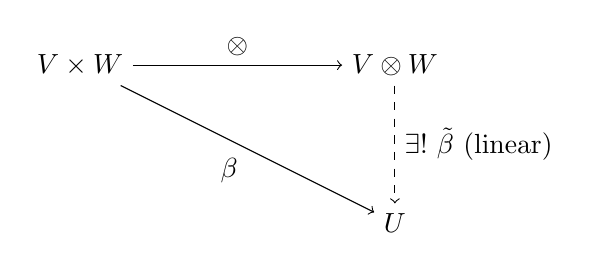
\begin{tikzpicture}[baseline=(current bounding box.center)]
  \node (VW) at (0,0) {$V\times W$};
  \node (T)  at (4,0) {$V\otimes W$};
  \node (U)  at (4,-2) {$U$};
  \draw[->] (VW) -- node[above]{$\otimes$} (T);
  \draw[->] (VW) -- node[below left]{$\beta$} (U);
  \draw[->,dashed] (T) -- node[right]{$\exists!\ \tilde\beta$ (linear)} (U);
\end{tikzpicture}

\]
\end{definition}

In words: \emph{bilinear maps out of $V\times W$ are the same thing as linear maps out of $V\otimes W$}.

\begin{proposition}[Uniqueness]
If $(T_1,\otimes_1)$ and $(T_2,\otimes_2)$ both satisfy Definition~\ref{def:tensor}, there is a unique
linear isomorphism $\phi:T_1\to T_2$ with $\phi(v\otimes_1w)=v\otimes_2w$.
\end{proposition}
\begin{proof}
Apply the universal property of $T_1$ to $\otimes_2$ to get $\phi:T_1\to T_2$, and that of $T_2$ to $\otimes_1$ to get
$\psi:T_2\to T_1$. Then $\psi\circ\phi$ is a linear map $T_1\to T_1$ compatible with $\otimes_1$, as is $\id_{T_1}$;
by the uniqueness clause they coincide. Likewise $\phi\circ\psi=\id_{T_2}$.
\end{proof}

% REWRITTEN: lead-in sentence added
\emph{Existence.} A tensor product always exists; here is the standard construction.
Let $F(V\times W)$ be the \emph{free vector space} on the \emph{set} $V\times W$: formal finite linear combinations
$\sum_a c_a\,[(v_a,w_a)]$ of the symbols $[(v,w)]$, which are declared linearly independent.
Let $N\subset F(V\times W)$ be the subspace spanned by all elements of the form
\begin{align*}
&[(v+v',w)]-[(v,w)]-[(v',w)], & &[(v,w+w')]-[(v,w)]-[(v,w')],\\
&[(\lambda v,w)]-\lambda[(v,w)], & &[(v,\lambda w)]-\lambda[(v,w)].
\end{align*}
Define $V\otimes W:=F(V\times W)/N$ and $v\otimes w:=[(v,w)]+N$. By construction $\otimes$ is bilinear.
Given a bilinear $\beta$, the linear extension of $[(v,w)]\mapsto\beta(v,w)$ to the free space kills $N$,
hence descends to the unique $\tilde\beta$ required. 

\begin{theorem}[Basis and dimension]\label{thm:tensorbasis}
If $(e_i)_{i\le n}$ and $(f_j)_{j\le m}$ are bases of $V$ and $W$, then $(e_i\otimes f_j)$ is a basis of $V\otimes W$.
In particular $\dim(V\otimes W)=nm$.
\end{theorem}
\begin{proof}[Proof sketch]
\emph{Spanning:} by bilinearity, $(v^ie_i)\otimes(w^jf_j)=v^iw^j\,e_i\otimes f_j$, and elements $v\otimes w$ span $V\otimes W$ by construction.
\emph{Independence:} for each pair $(k,l)$ the map $\beta_{kl}(v,w)=e^k(v)f^l(w)$ is bilinear, so it induces a linear
functional $\tilde\beta_{kl}$ on $V\otimes W$ with $\tilde\beta_{kl}(e_i\otimes f_j)=\delta_{ik}\delta_{jl}$. If $\sum c^{ij}e_i\otimes f_j=0$,
applying $\tilde\beta_{kl}$ gives $c^{kl}=0$.
\end{proof}

A general element is therefore $T=T^{ij}\,e_i\otimes f_j$. Elements of the form $v\otimes w$ are called
\emph{pure} (or decomposable); they are the exception rather than the rule: $e_1\otimes e_2+e_2\otimes e_1$ is not pure
(its coefficient matrix has rank $2$; pure tensors are exactly the rank-$1$ matrices). The same holds for
$e^{1}\otimes e^{2}+e^{2}\otimes e^{1}$, the kind of symmetric ``product'' used for metrics.

\begin{proposition}[Standard identifications (finite dimension)]
\begin{enumerate}
  \item $V\otimes\K\cong V$ and $(U\otimes V)\otimes W\cong U\otimes(V\otimes W)$ (associativity).
  \item $V^*\otimes W\cong\Hom(V,W)$ via $(\varphi\otimes w)(v)=\varphi(v)\,w$. In coordinates, $T^{i}{}_{j}\,e_i\otimes e^j$ is a matrix.
  \item $(V\otimes W)^*\cong V^*\otimes W^*$, and $V^*\otimes V^*\cong\{\text{bilinear forms on }V\}$. Hence a metric $g=g_{ij}e^i\otimes e^j$ is a tensor in $V^*\otimes V^*$.
\end{enumerate}
\end{proposition}

\begin{intuition}
The symbol $v\otimes w$ is a ``\emph{formal product that remembers nothing except bilinearity}''. You may
pull scalars out and distribute over sums, but you may \emph{not} simplify further: $v\otimes w\neq w\otimes v$,
and $v\otimes w$ is not a number or a vector, it is a new kind of object.
A concrete picture: $v\otimes w$ is the rank-one matrix $vw^{\mathsf T}$ (a table whose $(i,j)$ entry is $v^iw^j$);
a general tensor is a sum of such tables, i.e.\ any $n\times m$ table. The tensor product is thus the
\emph{space of all tables}, and the universal property says that any bilinear recipe can be evaluated by first
building the table and then applying a linear map to it.
\end{intuition}

% Section 2.3: Tensors of type $(\ell,k)$ | Part: 1 | Depends on: sec:vectors | Status: done | Original lines: 654-704
%!TEX root = ../../../main.tex
\subsection{Tensors of type $(\ell,k)$}\label{sec:tensortypes}
% REWRITTEN: notation E -> V (docs/NOTATION.md)
\begin{formal}[{tensors}]
A \emph{mixed tensor, $k$-covariant and $\ell$-contravariant} on $V$ is a multilinear map
\[
\tau:\underbrace{V\times\dots\times V}_{k}\times\underbrace{V^*\times\dots\times V^*}_{\ell}\to\R .
\]
The space of such tensors is $\TT{\ell}{k}(V)\cong \underbrace{V^*\otimes\dots\otimes V^*}_{k}\otimes\underbrace{V\otimes\dots\otimes V}_{\ell}$. Conventionally $\TT{0}{0}(V)=\R$ (scalars). Special cases:
\begin{center}
\begin{tabular}{@{}lll@{}}
\toprule
Space & Meaning & Components\\ \midrule
$\TT{0}{0}=\R$ & scalar & $\tau$\\
$\TT{0}{1}=V^*$ & covector & $f_i$\\
$\TT{1}{0}=(V^*)^*\cong V$ & vector & $v^i$\\
$\TT{0}{2}$ & bilinear form (\eg metric) & $g_{ij}$\\
$\TT{1}{1}$ & linear map $V\to V$ (via $A(v,\alpha)=\alpha(Av)$) & $A^i{}_j$\\
$\TT{1}{2}$ & (\eg torsion) & $T^i{}_{jk}$\\
$\TT{1}{3}$ & (\eg Riemann curvature) & $R^l{}_{ijk}$\\ \bottomrule
\end{tabular}
\end{center}
\end{formal}

\begin{intuition}[{a tensor is a coordinate-free machine; its components are a table}]
A tensor is a geometric object like a vector: it exists independently of any basis. It is a machine with $k$ ``vector hoppers'' and $\ell$ ``covector hoppers'' that returns a number. The components are just the table of outputs on basis elements:
\[
\tau^{i_1\dots i_\ell}{}_{j_1\dots j_k}=\tau\big(e_{j_1},\dots,e_{j_k},e^{i_1},\dots,e^{i_\ell}\big).
\]
So $\tau=\tau^{i_1\dots i_\ell}{}_{j_1\dots j_k}\;e^{j_1}\otimes\dots\otimes e^{j_k}\otimes e_{i_1}\otimes\dots\otimes e_{i_\ell}$.
\end{intuition}

\begin{formal}[{transformation rule of components}]
If $e'_i=A^j{}_ie_j$, the components of a tensor in the new basis are
\begin{equation}\label{eq:tensortransf}
\tau'^{\,i_1\dots i_\ell}{}_{j_1\dots j_k}=(A^{-1})^{i_1}{}_{a_1}\cdots(A^{-1})^{i_\ell}{}_{a_\ell}\;A^{b_1}{}_{j_1}\cdots A^{b_k}{}_{j_k}\;\tau^{a_1\dots a_\ell}{}_{b_1\dots b_k}.
\end{equation}
Each upper index is transformed with $A^{-1}$, each lower index with $A$. A physicist's definition: \emph{a tensor is an array of numbers that transforms like this under changes of basis}. (In the notes this appears with $B=A$.)
% AUTHOR-NOTE: "B" is never defined in this document (refers to the external lecture notes). Define it or drop the sentence. See docs/AUTHOR_NOTES.md #4.
\end{formal}

\begin{example}[{three ``matrices'', three different transformation laws}]
In matrix notation, with $M$ the component matrix and $A$ the change of basis:
\[
\TT{0}{2}\ (g_{ij}):\ M'=A^tMA,\qquad
\TT{1}{1}\ (A^i{}_j):\ M'=A^{-1}MA,\qquad
\TT{2}{0}\ (T^{ij}):\ M'=A^{-1}M A^{-t}.
\]
\emph{Test.} Dot product on $\R^2$, $g=\mathrm{diag}(1,1)$, and $A=\begin{pmatrix}1&-1\\1&1\end{pmatrix}$ from Section~\ref{sec:vs}: $g'=A^tA=\begin{pmatrix}2&0\\0&2\end{pmatrix}$: the new basis vectors are still orthogonal but have length $\sqrt2$. \emph{Test 2.} The trace of a $(1,1)$ tensor is invariant, $\tr(A^{-1}MA)=\tr M$, but $\tr(A^tMA)\neq\tr M$ in general: ``trace of a bilinear form'' is not a meaningful invariant without a metric.
\end{example}

% Section 2.4: Symmetric and antisymmetric tensors; contraction of tensors | Part: 1 | Depends on: sec:vectors | Status: done | Original lines: 705-741
%!TEX root = ../../../main.tex
\subsection{Symmetric and antisymmetric tensors; contraction of tensors}\label{sec:symcontr}
% REWRITTEN: the wedge product is defined once, in Section sec:ext (eq:wedge11); here it is only previewed.
A tensor $\tau\in\TT{0}{2}$ is \emph{symmetric} if $\tau(v,w)=\tau(w,v)$ and \emph{antisymmetric} if $\tau(v,w)=-\tau(w,v)$.
For covectors $\alpha,\beta$ the antisymmetric combination
\[
\alpha\otimes\beta-\beta\otimes\alpha
\]
will be called the \emph{wedge product} $\alpha\wedge\beta$ in Section~\ref{sec:ext}, where it is evaluated as
\eqref{eq:wedge11}: $(\alpha\wedge\beta)(v,w)=\alpha(v)\beta(w)-\alpha(w)\beta(v)$. Intuitively, this is the signed area of the
parallelogram spanned by $v,w$ as seen through the ``rulers'' $\alpha,\beta$. The notes use it in the area form of the sphere,
$r^2\sin\theta\,\dd\theta\wedge\dd\varphi$ (Example~\ref{ex:sphereareaform}).

\subhead{Contraction}
\begin{formal}[{contraction}]
The evaluation $V\times V^*\to\R$, $(v,f)\mapsto f(v)$ is bilinear, with $e_i,e^{j}\mapsto\delta^j{}_i$. Applying it to one covariant and one contravariant slot of a tensor gives a new tensor of type $(\ell-1,k-1)$. In components: set an upper and a lower index equal and sum,
\[
(c\tau)^{i_2\dots}{}_{j_2\dots}=\tau^{s\,i_2\dots}{}_{s\,j_2\dots}.
\]
This generalises the pairing \eqref{eq:pairing} of Section~\ref{sec:contraction}, which is the case $\tau=\omega\otimes v$.
\end{formal}
\begin{intuition}[{contraction = plug a vector-slot into a covector-slot}]
Think of connecting an output cable of one slot to the input of another and ``summing over all possible signals''. The result is lower in rank and \emph{still a tensor}. Examples: the trace $A^i{}_i$ of a linear map; the pairing $f_iv^i$; later the Ricci tensor $R^i{}_{ijk}$ and the scalar curvature.
\end{intuition}

% REORDERED: the exercises of this section (original L725-731) now close the section, in exercises.tex.

\begin{remark}[Three kinds of $2$-tensors]
A tensor in $\TT{0}{2}$ may be symmetric, antisymmetric, or neither; every one splits uniquely into a symmetric and an
antisymmetric part. A \emph{metric} is symmetric and non-degenerate (Section~\ref{sec:metric}); a \emph{$2$-form} is
antisymmetric (Section~\ref{sec:ext}); a general bilinear form such as $\dd x\otimes\dd y$ has both parts. The two parts
do different jobs -- one measures length, the other oriented area -- and the symmetric/antisymmetric bookkeeping
is made precise in Section~\ref{sec:wedgetensor}.
\end{remark}

% Section 2.5: The tensor algebra, and ``choose your relations'' | Part: 1 | Depends on: sec:vectors | Status: done | Original lines: 742-777
%!TEX root = ../../../main.tex
\subsection{The tensor algebra, and ``choose your relations''}\label{sec:tensoralgebra}
Write $V^{\otimes 0}=\K$, $V^{\otimes k}=V\otimes\cdots\otimes V$ ($k$ factors), of dimension $n^k$.

\begin{definition}[Tensor algebra]
$T(V)=\bigoplus_{k\ge0}V^{\otimes k}$, with the associative bilinear product induced by concatenation:
\[
 (v_1\otimes\cdots\otimes v_k)\cdot(w_1\otimes\cdots\otimes w_l)=v_1\otimes\cdots\otimes v_k\otimes w_1\otimes\cdots\otimes w_l .
\]
The unit is $1\in V^{\otimes0}=\K$. It is a \emph{graded algebra}: $V^{\otimes k}\cdot V^{\otimes l}\subset V^{\otimes(k+l)}$.
\end{definition}

\begin{theorem}[Universal property of $T(V)$]\label{thm:Tuniv}
For every unital associative algebra $A$ and every linear map $f:V\to A$ there is a unique algebra homomorphism
$\bar f:T(V)\to A$ with $\bar f|_V=f$, namely $\bar f(v_1\otimes\cdots\otimes v_k)=f(v_1)f(v_2)\cdots f(v_k)$.
\end{theorem}

This says $T(V)$ is the \emph{free} associative algebra generated by $V$: no relations are imposed on products.
Consequently every algebra generated by $V$ is a quotient $T(V)/\mathcal I$ for a two-sided ideal $\mathcal I$ of relations.

\begin{intuition}
Think of $T(V)$ as ``words'' in the ``alphabet'' $V$: $e_1e_2e_1$ and $e_1e_1e_2$ are different words.
Imposing a relation such as ``$vv=0$'' or ``$vv=|v|^2$'' is like declaring certain words equivalent and so
collapsing the (enormous) free algebra to a smaller one. Different relations give different geometries:
\begin{center}
\begin{tabular}{lll}
relation on $v\in V$ & resulting algebra & geometric content\\\hline
$v\otimes w=w\otimes v$ & symmetric algebra $S(V)$ & polynomials\\
$v\otimes v=0$ & exterior algebra $\bigwedge V$ & oriented areas, volumes\\
$v\otimes v=Q(v)$ & Clifford algebra $\Cl(V,Q)$ & lengths, angles, areas, rotations
\end{tabular}
\end{center}
\end{intuition}

% Section 2 (exercises): Exercises | Part: 1 | Depends on: sec:vectors | Status: done | Original lines: 725-731
%!TEX root = ../../../main.tex
% REORDERED: moved from the middle of sec:symcontr to the end of the section; notation E -> V, m -> n.
\begin{exercises}
\begin{enumerate}[nosep]
\item Show that $\dim\TT{\ell}{k}(V)=n^{k+\ell}$.
\item For $V=\R^3$, $e'_1=2e_1$, $e'_2=e_2$, $e'_3=e_3+e_1$: compute the dual basis change, and the components of $f=e^{1}+e^{3}$ in the new basis.
\item Show that the identity map of $V$ is the $(1,1)$ tensor $\delta^i{}_j$ with the same components in every basis.
\end{enumerate}
\end{exercises}

